%\documentclass[xcolor=dvipsnames]{beamer}
\documentclass{standalone}

%\setbeamertemplate{navigation symbols}{}%remove navigation symbols
\usepackage{stmaryrd}
\usepackage{amssymb,amsthm,amsmath,amsxtra}
\usepackage{tikz}
\usetikzlibrary{arrows,calc,automata,shadows,backgrounds,positioning,intersections,fadings,decorations.pathreplacing,shapes,decorations,matrix}

\newcommand{\PP}{\mathbb P}

\begin{document}

    %\includegraphics[scale=.5]{monodromy.pdf}
    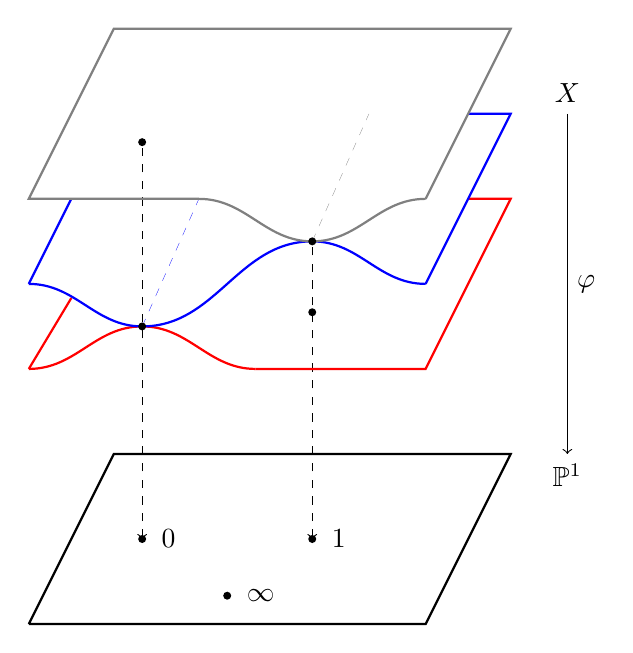
\begin{tikzpicture}[scale=.36]
      % dashed
      \draw[blue,ultra thin,dashed] (4,10.5)--(6,15);
      \draw[gray,ultra thin,dashed] (10,13.5)--(12,18);
      \draw[<-,black,thin,dashed] (4,3)--(4,17);
      \draw[<-,black,thin,dashed] (10,3)--(10,13.5);
      % ComplexPlane
      \draw[thick] (0,0)--(14,0)--(17,6)--(3,6)--(0,0);
      % sheet 1
      \draw[thick,red] (8,9)--(14,9)--(17,15)--(15.5,15);
      % sheet 2
      \draw[blue,thick] (0,12)--(1.5,15);
      \draw[blue,thick] (15.5,18)--(17,18)--(14,12);
      % sheet 3
      \draw[gray,thick] (6,15)--(0,15)--(3,21)--(17,21)--(14,15);
      % branching
      \draw[red,thick] (0,9)--(1.5,11.5);
      \draw[red,thick] (0,9) to[out=0,in=-180] (4,10.5);
      \draw[red,thick] (4,10.5) to[out=0,in=-180] (8,9);
      \draw[blue,thick] (0,12) to[out=0,in=-180] (4,10.5);
      \draw[blue,thick] (4,10.5) to[out=0,in=-180] (10,13.5);
      \draw[blue,thick] (10,13.5) to[out=0,in=-180] (14,12);
      \draw[gray,thick] (6,15) to[out=0,in=-180] (10,13.5);
      \draw[gray,thick] (10,13.5) to[out=0,in=-180] (14,15);
      % points
      \fill [black] (4,3) circle (4pt);
      \node at (4,3) [label=right:$0$] {};
      \fill [black] (10,3) circle (4pt);
      \node at (10,3) [label=right:$1$] {};
      \fill [black] (10,11) circle (4pt);
      %\node at (12.5,11) {$x=1/2$};
      \fill [black] (4,10.5) circle (4pt);
      %\node at (6.5,10.5) {$x=0$};
      \fill [black] (4,17) circle (4pt);
      %\node at (7,17) {$x=-3/2$};
      \fill [black] (10,13.5) circle (4pt);
      %\node at (13,13.5) {$x=-1$};
      \fill [black] (7,1) circle (4pt);
      \node at (7,1) [label=right:$\infty$] {};
      % misc
      %\node[red] at (-1,9) {$1$};
      %\node[blue] at (-1,12) {$2$};
      %\node[gray] at (-1,15) {$3$};
      \node at (19,18.75) {$X$};
      \node at (19,5.25) {$\PP^1$};
      \draw[black,->] (19,18) to node[right]{$\varphi$} (19,6);
    %\node at (22,12) {z=\phi(x)=2x^3+3x^2$};
      %\node at (24,12) {$\phi(x)=2x^3+3x^2$};
    \end{tikzpicture}
\end{document}
